% Document template
\documentclass	[a4paper,11pt, hidelinks]{article}

% Support for including graphics
\usepackage		{graphicx}

% Support for creating PS/PDF graphics
\usepackage		{pgf}

% Support for creating plots
\usepackage		{pgfplots}

% Support for creating drawings
\usepackage		{tikz} 

% Support for extensive control of page headers and footers
\usepackage		{fancyhdr}

% Support for hypertext
\usepackage		{hyperref}

% Support for adding background
\usepackage		{background}

% Support for tables with adjustable-width columns
\usepackage		{tabularx}

% Support for publication quality tables
\usepackage		{booktabs}

% Support for tabular cells spanning multiple rows
\usepackage		{multirow}

% Support for Driver-independent color extensions
\usepackage		{xcolor}

% Support for hyphenation for letterspacing, underlining
\usepackage		{soul}	

% Support for date and time
\usepackage		{datetime}

% AMS Maths package
\usepackage		{amsthm}
\usepackage		{amssymb}

\theoremstyle	{definition}
\newtheorem		{axiom}{Axiom}
\newtheorem		{theorem}{Theorem}
\newtheorem		{corollary}{Corollary}[theorem]
\newtheorem		{lemma}{Lemma}[theorem]
\newtheorem		{definition}{Definition}

% Create vertical text
\SetBgContents	{}
\SetBgPosition	{current page.west}
\SetBgVshift	{-1.8cm}
\SetBgOpacity	{1}
\SetBgAngle		{90.0}
\SetBgScale		{1.2}
\SetBgAnchor	{}

% Set creation date
\newdate		{date}{29}{08}{2019}
\date			{\displaydate{date}}

% Remove paragraph indent
\setlength		{\parindent}{0em}

% Add after paragraph spacing
\setlength		{\parskip}{0.5em}

% Set images path
\graphicspath	{{images/}}

% Clear all header and footers
\fancyhf		{}

% Remove the header rule
\renewcommand	{\headrulewidth}{0pt}

% Set page number in right footer
\rfoot			{\thepage}							

% Set header
\chead			{}

% Set left footer
\lfoot			{}
\AtEndDocument	{\lfoot{}}

% Set page styles as fancy
\pagestyle		{fancy}

% Set document Title
\title{Predictive Modelling for HCI \& Ergonomics}

% Document
\begin{document}
\maketitle
\thispagestyle{fancy}

\begin{large}How do we extend Fitt’s Law to two or more dimensional target tasks with complex factors like usage of shape, color and other visual attributes of the target?
\end{large}

\section{Overview of the Project}
One of the well known and robust methods, Fitt’s law identifies an effective model of human psychomotor behavior in the context of Human-Computer interaction. It tells us how time required to rapidly move to a target area is a function of the ratio between the distance to the target and the width of the target.\cite{fitts1954information}

\begin{figure}[h]
  \center
  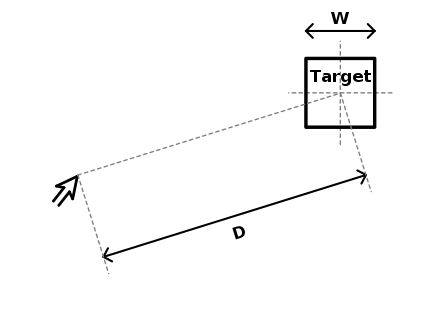
\includegraphics[width=0.5\textwidth]{images/440px-Fitts_Law}
\end{figure}

$$ MT = a + b \log_{2} \frac{2D}{W} $$

The model generalizes the act of pointing and can be extended to either physically touching an object or virtually pointing on a computer monitor. This in fact eventually led to the factor leading to the mouse’s commercial introduction by Xerox over the joystick or any other directional movement input device.\cite{stuart_crt} Fitt’s law has played an important role in understanding and designing user interfaces. However, the law is constrained to only one dimension and does not account for factors like usage of color, contrast, etc. due to their complexity. Through this project, \textit{the aim is to design tools to study gaps in various predictive models but primarily Fitt’s law for two-dimensional target acquisition tasks}.

\section{Objectives and Activities}
\textbf{To design, prototype and conduct a series of experiments to identify and study complex factors for two-dimensional target acquisition tasks.}

\begin{enumerate}
  \item \textbf{Literature Review.} Studying existing predictive models for HCI: Fitts, Welford, Steering law, etc.
  \item \textbf{Design of experiments and Prototyping.} Identification of complex factors; and developing a web-based app to facilitate a series of experiments to collect user psychomotor behavior.
  \item \textbf{Performing Experiment.} Recruiting participants, and carrying out the experiments with the participants, and prepare data that can be studied to model the extension of Fitt’s law.
  \item \textbf{Documentation.} Documenting and presenting the results of the study.
\end{enumerate}

\section{Scope of the Project}
The current scope of the project is limited to experiment design and preliminary testing of the same with participants in a supervised environment.  This will eventually go towards deploying a real web app to carry out such experiments at large magnitude and model the extended Fitt’s law.

\section{Expected Skills/Interests}
\begin{enumerate}
  \item Interest in HCI and computational models.
  \item Know-how of empirical and quantitative investigation.
  \item Experience with HTML and JS to build interactive web pages.
  \item Experience with p5.js or similar visual prototyping tools would be an advantage.
\end{enumerate}

\section{Learning Outcomes}
\begin{enumerate}
  \item Understanding of the predictive psychomotor models that facilitate groundwork for designing user interfaces.
  \item Using prototyping to design experiments to conduct quantitative research.
  \item Relationships between complex factors that influence human motor movement for two-dimensional target tasks; Computational modeling.
\end{enumerate}

\section{Other Details}
\begin{itemize}
  \item This project does not involve travel.
  \item Student limit: 20 maximum.
\end{itemize}

\section{Further Reading}
\begin{itemize}
	\item R. V. L. Hartley (July 1928). "Transmission of Information" (PDF). Bell System Technical Journal.
	\item Drury, C. G. (1971). "Movements with lateral constraint". Ergonomics. 14 (2): 293–305. doi:10.1080/00140137108931246. PMID 5093722.
	\item Johnny Accot and Shumin Zhai (1997). Beyond Fitts' law: models for trajectory-based HCI tasks. Proceedings of ACM CHI 1997 Conference on Human Factors in Computing Systems, pp. 295–302. http://doi.acm.org/10.1145/258549.258760
\end{itemize}

\bibliography{ref.bib}
\bibliographystyle{plain}

\end{document}
